%--------------------------------------
% Create title frame
\titleframe

%--------------------------------------
% Table of contents
\begin{frame}{Overview}
  \setbeamertemplate{section in toc}[sections numbered]
  \tableofcontents[hideallsubsections]
\end{frame}



%--------------------------------------


\begin{frame}{Overview}
\begin{itemize}
    \item Concept of stability
    \begin{itemize}
        \item General concept
        \item In power systems
    \end{itemize}
    \item Why do we need stability?
    \item Voltage instability and voltage collapse
    \begin{itemize}
        \item Impact of power flows on voltages
        \item Concept of nose curve
        \item Examples of voltage instabilities
    \end{itemize}
    \item (Some) counter-measures
    \begin{itemize}
        \item Network reinforcement
        \item Voltage regulation
    \end{itemize}
    \item Impact of renewable energy resources (RES)
    \begin{itemize}
        \item Reverse power flows in distribution systems
        \item Duck curve
    \end{itemize}
    \item What did we learn?
\end{itemize}
\end{frame}

\section{The concept of stability}
\begin{frame}{General concept}
\begin{quote}
    \textbf{If a system has the property that it will get back into the equilibrium state 
    again after moving away from its equilibrium state, then it is stable.} \cite{keviczky2018stability}
\end{quote}
\vspace{0.5cm}
\begin{center}
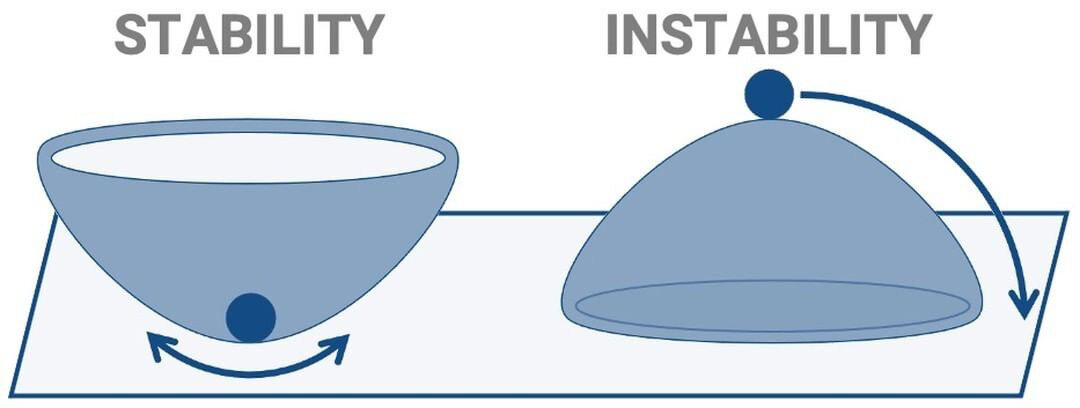
\includegraphics[width=0.7\textwidth]{images/ConceptOfStability.png}
\end{center}
\end{frame}

\begin{frame}[allowframebreaks]{In power systems}
\begin{quote}
    \textbf{Power system stability is the ability of an electric power system, 
    for a given initial operating condition, to regain a state of operating equilibrium 
    after being subjected to a physical disturbance, with most system variables bounded 
    so that practically the entire system remains intact.} \cite{hatziargyriou2020definition}
\end{quote}
\vspace{0.5cm}
\begin{center}
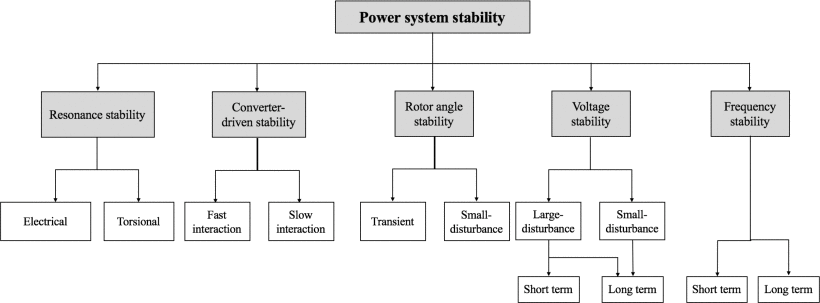
\includegraphics[width=0.9\textwidth]{images/ClassificationStability.png}
\end{center}
\end{frame}


\section{Why do we need stability?}

\begin{frame} {Key points}
\begin{itemize}
    \item We often take electricity as a simple commodity.
    \item But the electric power system is one of the most complex and largest man-made system.
    \item The chances of system failures are very high taking into account the impact of external factors and rapid changes in system's state.
    \item However, power systems are very reliable (operated 24h/24h 7d/7d and only a few hours of power outages per year!).
    \item But when instabilities occur, it can lead to blackouts with huge financial and societal consequences.
\end{itemize}
\end{frame}

\begin{frame}{Tokyo 1987}
\begin{itemize}
    \item Unexpected load increase and presence of constant power devices (air conditioners) led to a voltage collapse.
\end{itemize}
\vspace{0.5cm}
\begin{center}
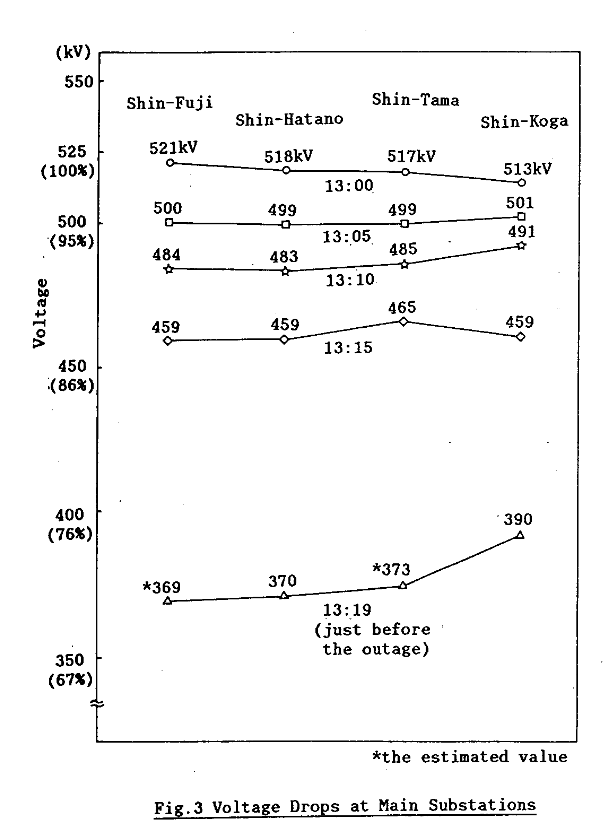
\includegraphics[width=0.4\textwidth]{images/TokyoCollapse.png}
\end{center}
\vspace{0.5cm}
\begin{quote}
    \textbf{8 GW lost} and \textbf{2.8M customers impacted} \cite{ohno2006tokyo, kurita1988power}
\end{quote}
\end{frame}

\begin{frame}{Canada/Northeast USA 2003}
\begin{itemize}
    \item Initial problem: not enough reactive power reserve. Hot weather and large consumption led to transmission lines overloading and eventually sagging into trees, further deteriorating the initial problem.
    \item A cascading event caused the tripping of hundreds of lines and generating units.
\end{itemize}
\vspace{0.5cm}
\begin{center}
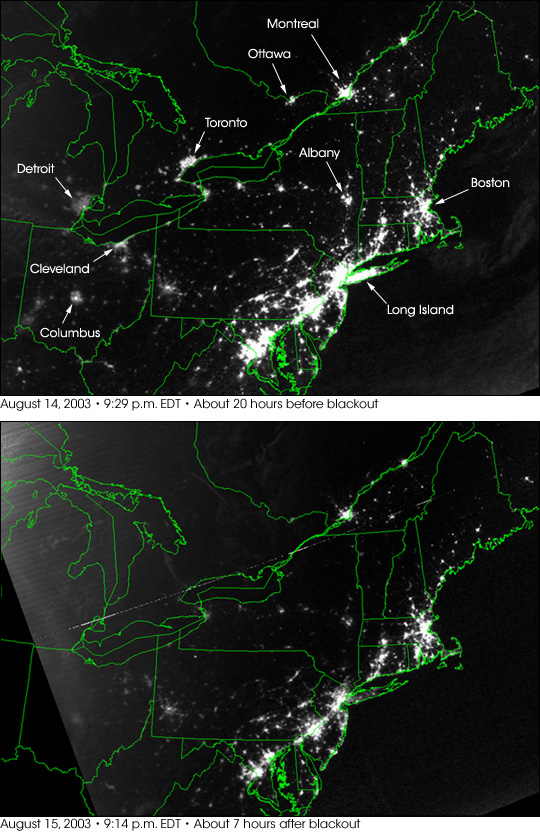
\includegraphics[width=0.4\textwidth]{images/USABlackOut.png}
\end{center}
\vspace{0.5cm}
\begin{quote}
    \textbf{63 GW lost} and \textbf{50M customers impacted} and \textbf{Estimated cost above \$5 Billion}
\end{quote}
\end{frame}

\begin{frame}{Europe 2006}
\begin{itemize}
    \item Disconnection of a transmission line in Germany for the transport of a ship approved by the local TSO.
    \item The local TSO approved to advance the disconnection later that day, but the commercial flows remained unchanged.
    \item Some lines were critically loaded because of the line disconnection and a fast increase of load consumption led to a cascading event.
    \item European interconnected network has been split into 3 islands.
\end{itemize}
\vspace{0.5cm}
\begin{center}
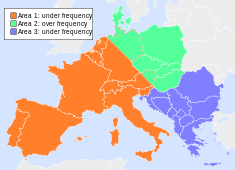
\includegraphics[width=0.4\textwidth]{images/EuropeBlackOut.png}
\end{center}
\vspace{0.5cm}
\begin{quote}
    \textbf{14.5 GW lost} and \textbf{15M customers impacted} \cite{li2007analysis}
\end{quote}
\end{frame}

\begin{frame}{Brazil 2023}
\begin{itemize}
    \item False operation of a relay protection system led to a 500kV line disconnection.
    \item The Energy Management System did not operate properly.
\end{itemize}
\vspace{0.5cm}
\begin{quote}
    \textbf{19 GW lost}
\end{quote}
\vspace{0.5cm}
\hrule
\vspace{0.5cm}
\begin{itemize}
    \item Every time a black-out happened, lessons have been learned, and new rules have been put in place.
    \item Nonetheless, due to the system complexity, new complex phenomena occur that power system engineers try to understand.
    \item In the following, we'll dive into the mechanisms of voltage instability.
\end{itemize}
\end{frame}


\section{Voltage instability and voltage collapse}

\begin{frame}{Impact of power flows on voltages}
Consider a simple radial system.
\vspace{0.5cm}
\begin{center}
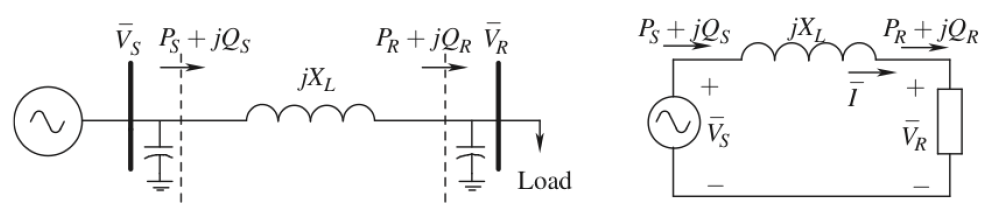
\includegraphics[width=\textwidth]{images/RadialSystem.png}
\end{center}
Assuming no transmission-line losses:
$$S_S = P_S + jQ_S = V_S e^{j \delta_S} \left(\frac{V_S e^{-j \delta_S} - V_R e^{-j \delta_R}}{X}\right) e^{j\frac{\pi}{2}}$$
$$S_R = P_R + jQ_R = V_R e^{j \delta_R} \left(\frac{V_S e^{-j \delta_S} - V_R e^{-j \delta_R}}{X}\right) e^{j\frac{\pi}{2}}$$
\end{frame}

\begin{frame}{Impact of power flows on voltages}
If we define $\delta = \delta_S-\delta_R$, we have:
$$P_R = P_S = \frac{V_S V_R}{X_L}\sin \delta$$
$$Q_{R} = \frac{V_S V_R \cos \delta}{X_L} - \frac{V^2_R}{X_L}$$
$$Q_{S} = \frac{V_S^2}{X_L} - \frac{V_S V_R \cos \delta}{X_L}$$
\textbf{Question:} What is the sign of $Q_S$ if $V_S>V_R$. What about $Q_R$?
\hrule
From the expression of $Q_{R}$, dividing both sides by $\frac{V_R^2}{X_L}$, we get:
$$\frac{V_R}{V_S} = \cos \delta \left(\frac{1}{1+\frac{Q_R}{V^2_R/X_L}}\right)$$
Assuming $P_S>>0$ and $V_R \approx V_S \approx 1$, it leads to $\delta >> 0 \rightarrow \cos \delta << 1$.
\textbf{Question:} What would be the sign of $Q_R$ to keep $\frac{V_R}{V_S}\approx 1$ as you increase $P_S$?
\end{frame}

\begin{frame}{Impact of power flows on voltages}
Consider the following radial system, and the associated phasor diagram for which we consider $V_R = 1 e^{j0}, V_S = 1 e^{j\delta}$.
\begin{center}
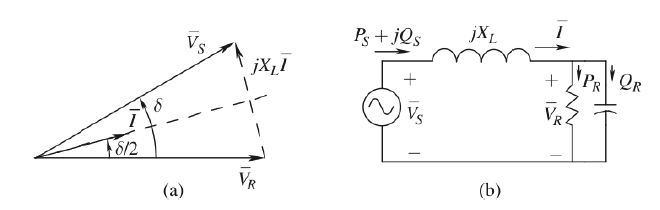
\includegraphics[width=0.9\textwidth]{images/RadialSystem2.png}
\end{center}
Considering Kirchhoff's Laws, one has:
$$\bar{V}_S = \bar{V}_R + j X_L \bar{I} \Rightarrow \bar{I} = \frac{e^{j \delta}-1}{j X_L} = \frac{2 \sin(\delta/2)}{X_L} e^{j(\delta/2)}$$
As $\bar{I}$ is leading $\bar{V}_R$, $Q_R = |\bar{V}_R| |\bar{I}| \sin(-\delta/2)$ is negative. $Q_S$ is positive and one can write:
$$Q_S = -Q_R$$
\textbf{The larger $\delta \rightarrow P_{s \rightarrow r}$, the larger $Q_R$ and $Q_S$ to maintain $V_R = V_S = 1$}
\end{frame}

\begin{frame}{Impact of power flows on voltages}
\textbf{Question:} Where does the reactive power go?
\begin{itemize}
    \item Total reactive power loss:
    $$Q_S-(-Q_S) = 2 Q_S$$
    \item Line current:
    $$\bar{I} = \frac{2 \sin(\delta/2)}{X_L} e^{j(\delta/2)}$$
    \item Reactive power consumed by the line:
    $$X_L |\bar{I}|^2 = \frac{4}{X_L} \sin(\delta/2)^2 = 2 Q_S$$
\end{itemize}
\end{frame}

\begin{frame}{Key points}
\begin{itemize}
    \item For HV systems, we usually assume:
    $P_{s \rightarrow r} \propto (\delta_s - \delta_r)$
    \item And $Q_{s \rightarrow r} \propto (V_s-V_r)$
    \item Lines are mostly inductive so they consume reactive power.
    \item Therefore, voltage control is done locally to avoid transferring reactive power over long distances.
\end{itemize}
\end{frame}

\begin{frame}{Concept of nose curve}
Consider again the following simple radial system.
\begin{center}
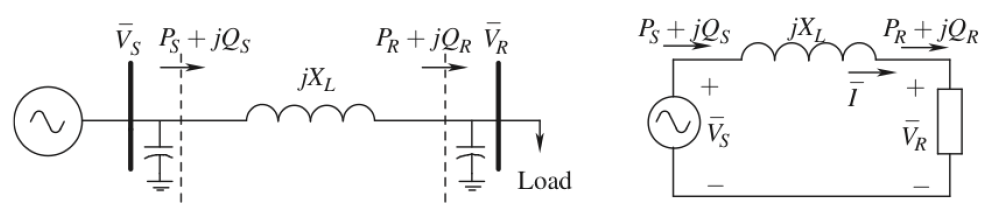
\includegraphics[width=0.9\textwidth]{images/RadialSystem.png}
\end{center}
Consider $Q_R = 0 \Rightarrow \frac{V_S V_R \cos \delta}{X_L} - \frac{V^2_R}{X_L} = 0 \Rightarrow V_S \cos \delta = V_R$
We know $P_R = \frac{V_SV_R}{X_L}\sin \delta$, substituing the previous results in the expression of $P_R$ gives:
$$P_R = \frac{V_S^2}{X_L}\sin \delta \cos \delta = \frac{V_S^2}{2 X_L}\sin (2\delta)$$
We can determine the maximum transmissible power by setting the partial derivative to 0:
$$\frac{\partial P_R}{\partial \delta}(\delta^{max}) = \frac{V_S^2}{X_L}\cos (2\delta^{max}) = 0 \Rightarrow \delta^{max} = \frac{\pi}{4}$$
\end{frame}

\begin{frame}{Concept of nose curve}
Replacing $\delta$ by $\delta^*$ in the equation of $P_R$, we have:
$$P_{R}^{max} = \frac{V_S^2}{2 X_L}$$
and
$$V_R \approx 0.7 V_S$$
\textbf{Question:} How can we increase the maximum transmissible power through a line?
\hrule
One can derive a relationship such that $\frac{V_R}{V_S} = f(\frac{P_R X_L}{V_S^2})$. Consider $y = \frac{V_R}{V_S}$ and $x = \frac{P_R X_L}{V_S^2}$, one has (trust me):
$$y = \sqrt{\frac{1}{2}\pm \sqrt{\frac{1}{4}-x^2}}$$
We verify that $y$ has a unique solution when $x = \frac{1}{2} \Rightarrow P_R = \frac{V_S^2}{2 X_L}$, which is the nose of the curve. There is no solution for $P_R > \frac{V_S^2}{2 X_L}$ and two solutions for $P_R < \frac{V_S^2}{2 X_L}$.
\end{frame}

\begin{frame}{Concept of nose curve}
Let us consider different load characteristics:
$$P_{constant} \Rightarrow P_R = C_P \Rightarrow x = c_P$$
$$I_{constant} \Rightarrow \frac{P_R}{V_R} = C_I \Rightarrow y = c_I x$$
$$Z_{constant} \Rightarrow \frac{P_R}{V^2_R} = C_Z \Rightarrow y = c_Z \sqrt{x}$$
The operating point is where the load characteristic crosses the \emph{PV curve}.
\begin{center}
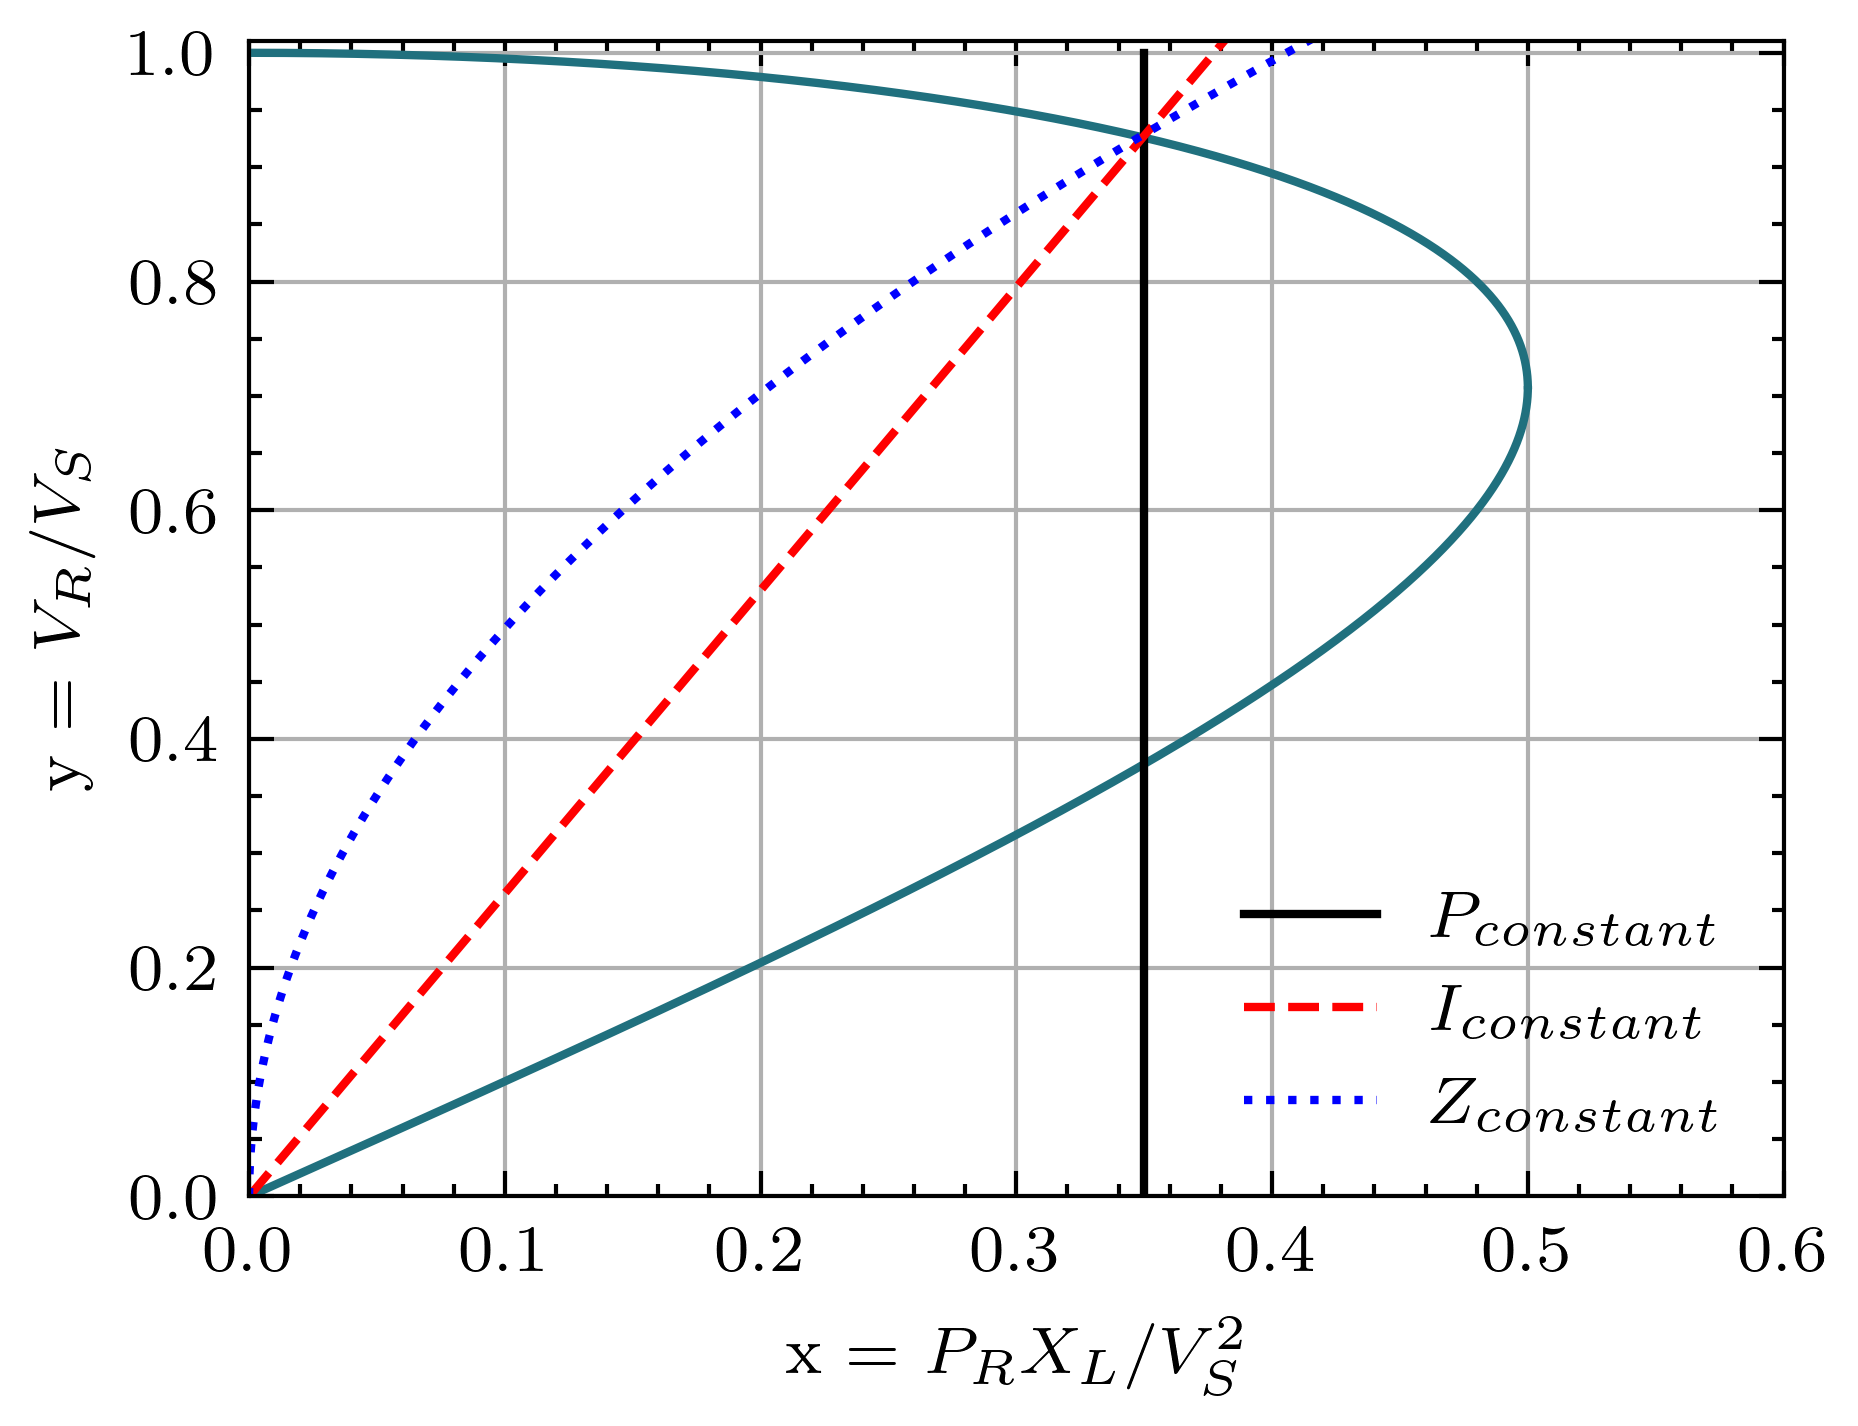
\includegraphics[width=0.6\textwidth]{images/NoseCurve.png}
\end{center}
\textbf{Question:} Where does that shape come from?
\end{frame}

\begin{frame}{Concept of nose curve}
$$P_R = V_R I \cos{\phi} = \frac{V_SV_R}{X_L}\sin \delta$$
Let us consider $\cos{\phi} = 1$ (unity power factor), and $X_L=1$ as well as $V_S=1$.
$$I = \frac{V_S}{X_L}\sin \delta = \sin \delta$$
$$Q_S = \frac{V_S^2}{X_L} - \frac{V_S V_R \cos \delta}{X_L} = 1-V_R \cos \delta$$
Since $Q_R = 0$, you know that $Q_S = X_L I^2 = I^2 \Rightarrow \frac{-I^2+1}{\cos \delta} = V_R$.
Consider the Taylor expansion of $\sin \delta \approx \delta$ and $\cos \delta \approx 1-\frac{\delta^2}{2}$ for $\delta \approx 0$, we have
$$V_R \approx \frac{(1-I^2)}{(1-I^2)+I^2/2}$$
\end{frame}

\begin{frame}{Concept of nose curve}
\begin{center}
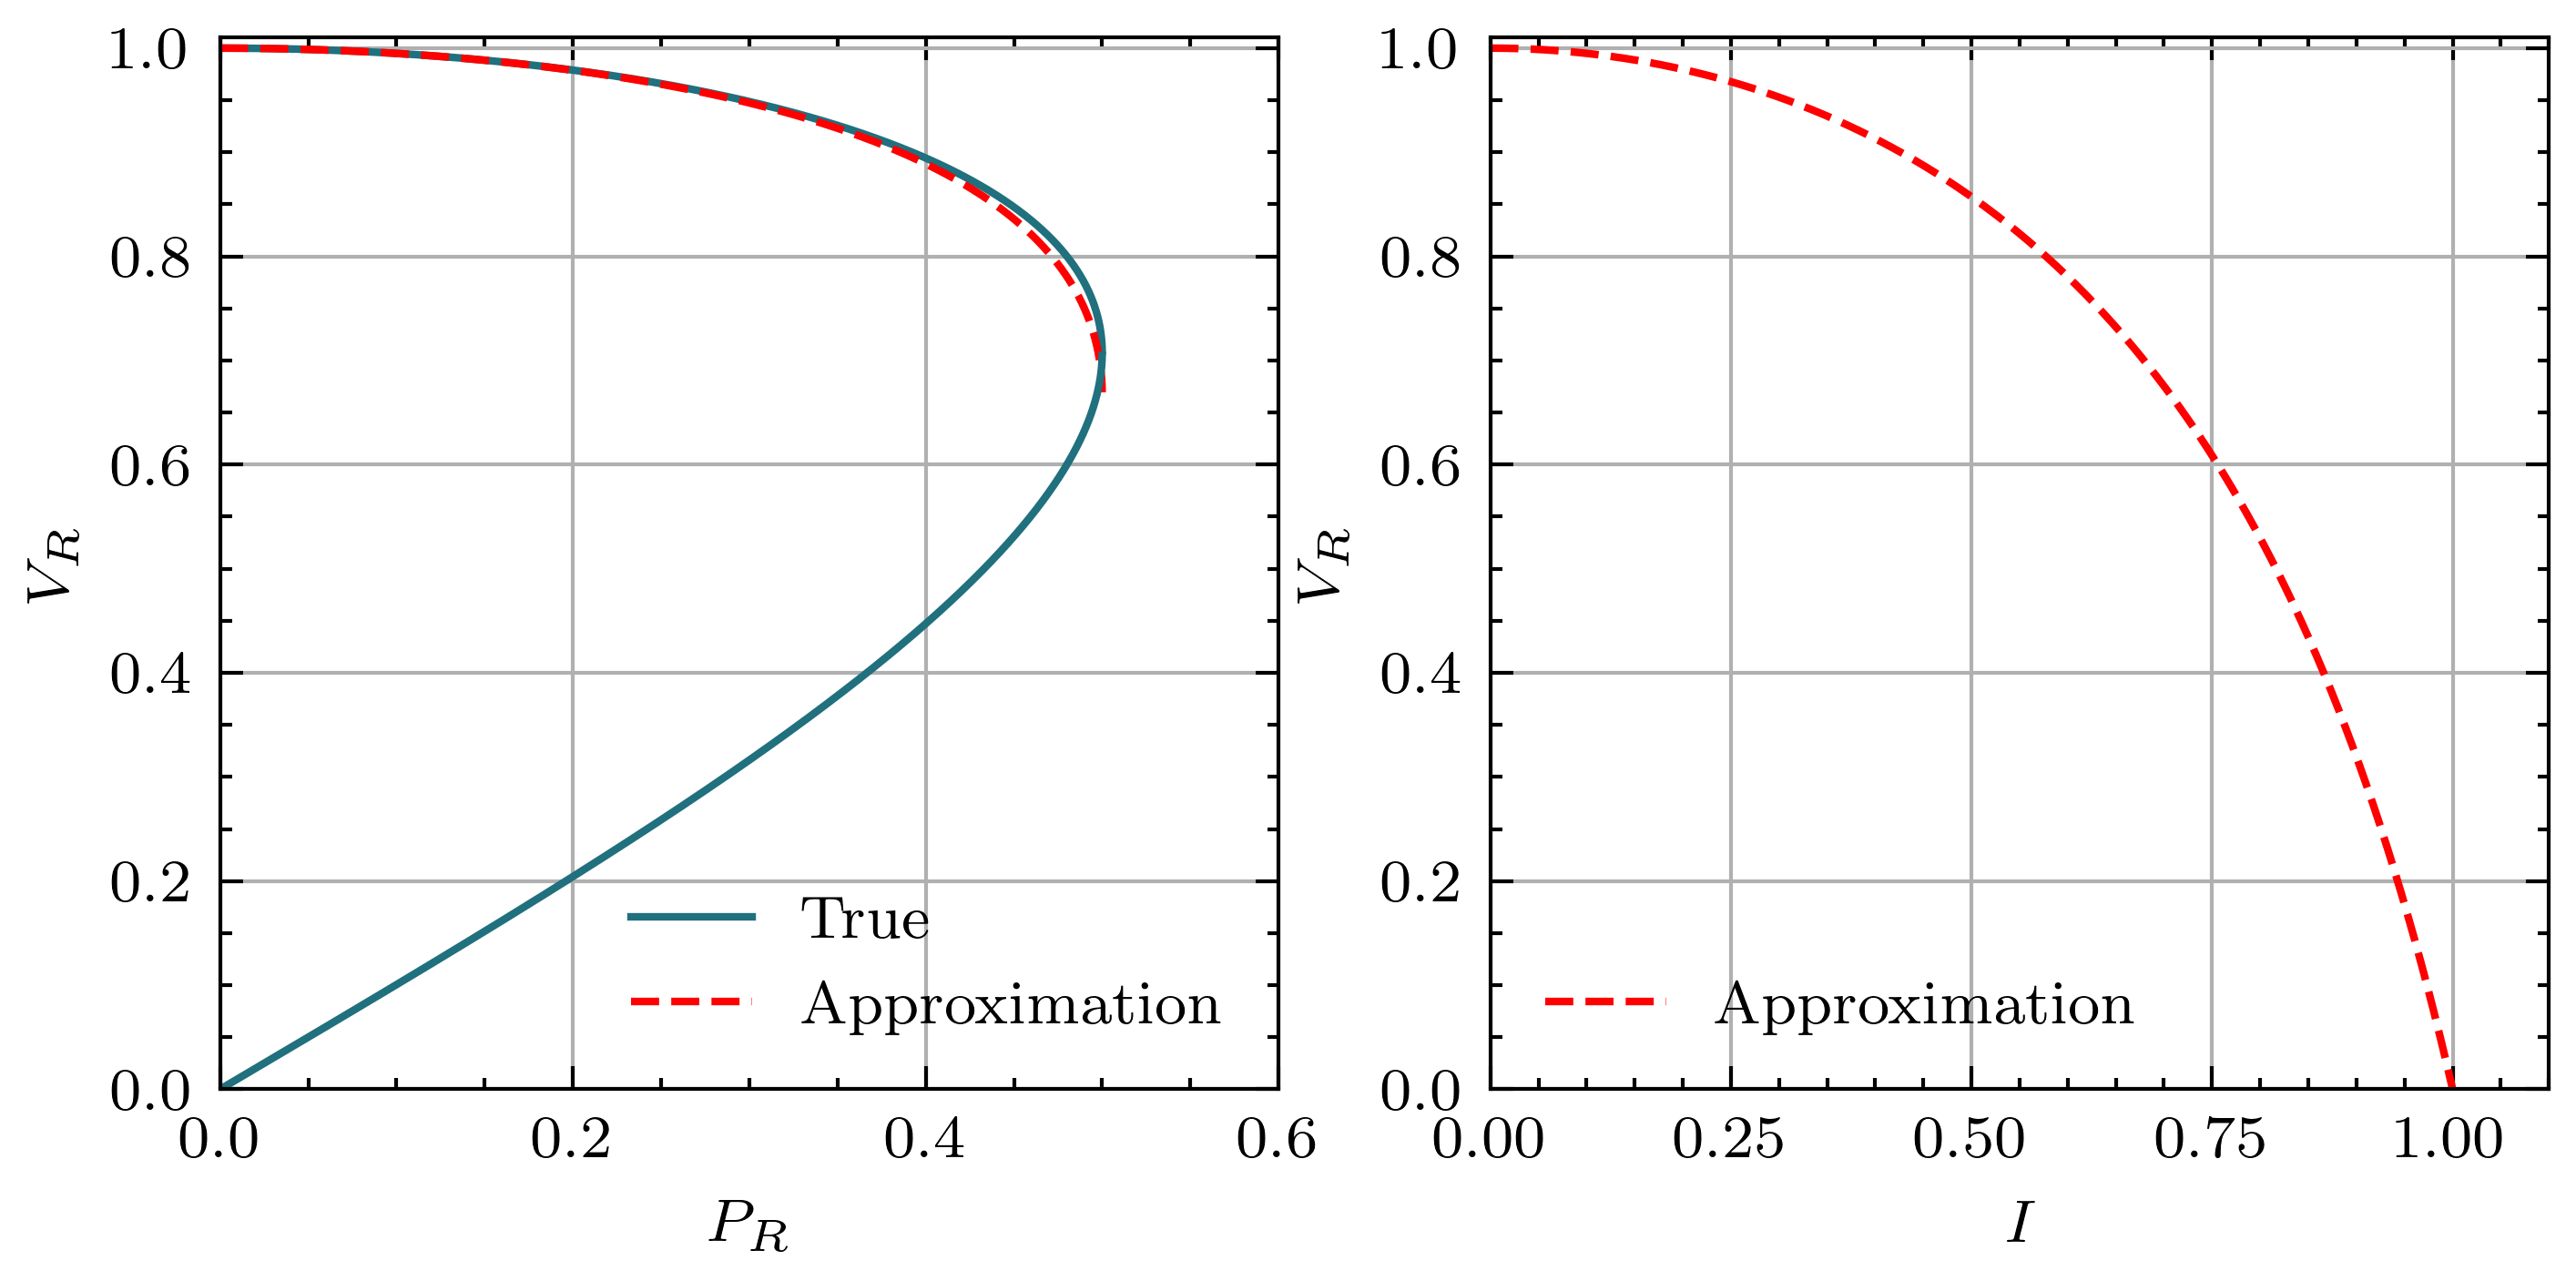
\includegraphics[width=0.8\textwidth]{images/NoseCurveApprox.png}
\end{center}
Since $I=\sin \delta \leq 1$, which implies that $(1-I^2) \geq 0$ and therefore $V_R$ decreases when $I$ increases. But after a given value of $I$, $V_R$ decreases faster than $I$ increases. Since $P_R = V_R I \cos{\phi}$, there is a maximum power transmissible.
It does so because the line is inductive, and thus consumes reactive power. The larger the current, the larger the reactive power consumed by the line, which pulls the voltage down.
\textbf{Question:} Is that everything we need to know about nose curves?
\end{frame}

\begin{frame}{Concept of nose curve}
\textbf{NO}
When you consider $\cos \phi \neq 1$ (the load consumes or produces reactive power), you get more complex nose curves \cite{van2007voltage}.
\begin{center}
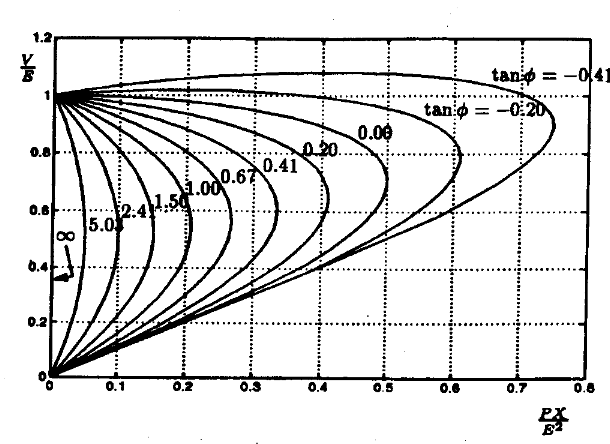
\includegraphics[width=0.6\textwidth]{images/TrueNoseCurve.png}
\end{center}
The ideas previously developed still stand, except that now the load can:
\begin{itemize}
    \item \emph{improve} the voltage profile by providing reactive power and thus compensating the reactive power consumed by the line,
    \item or \emph{worsen} it by further consuming reactive power.
\end{itemize}
\end{frame}

\begin{frame}{Key points}
\begin{itemize}
    \item There's a maximum transmissible power ($P_{R}^{max} = \frac{V_S^2}{2 X_L}$ for load with $\cos \phi = 1$).
    \item Inductive character of the line which consumes reactive power (influence of $X_L$)
\end{itemize}
\emph{How to increase $P_{R}^{max}$?}
\begin{itemize}
    \item By increasing the source voltage $V_S$,
    \item By decreasing $X_L$ (adding lines in parallel),
    \item By producing reactive power at the load side to compensate for the reactive power consumed by the line.
\end{itemize}
\end{frame}

\begin{frame}{Examples of voltage instabilities}
\emph{Long-term instabilities}
On-load tap changers (OLTCs) change the turn ratio of the transformers feeding the distribution systems to keep the voltages on the secondary side as close as possible to a given setpoint.
Let us consider the following circuit, where the primary side of the transformer is the high voltage network, and the secondary side is the medium voltage network.
The load on the secondary side is represented by a constant conductance $G$, consuming active power.
The voltage on the primary side is controlled by a synchronous generator. $V_g$ is kept constant as long as the reactive power limits of the generator are not reached.
\begin{center}
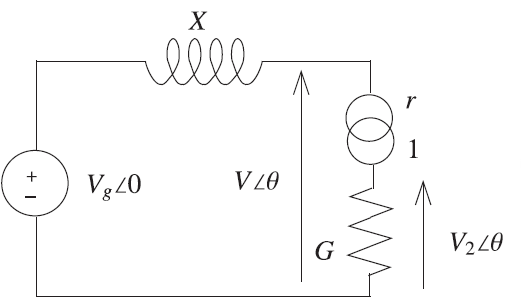
\includegraphics[width=0.6\textwidth]{images/OLTC.png}
\end{center}
\end{frame}

\begin{frame}{Examples of voltage instabilities}
We assume an ideal transformer: $\frac{V}{V_2} = r$, $\frac{I_2}{I} = r$.
The load characteristic seen from the primary side becomes $P_G = G\left(\frac{V}{r}\right)^2$, with $P_G$ the power consumed by the conductance $G$.
Now, imagine one wants to keep $V_2 = V_2^o$, if $V \searrow \Rightarrow r \searrow$. Indirectly, by decreasing $r$, the OLTC tries to restore the load (since it increases $V_2$ and $P_G = G V_2^2 = G\left(\frac{V}{r}\right)^2$).
Two different scenarii:
\begin{itemize}
    \item 1) $\frac{V}{r}$ converges towards $V_2^o$, the load is restored.
    \item 2) $\frac{V}{r}$ never converges towards $V_2^o$ and $V$ collapses.
\end{itemize}
\end{frame}

\begin{frame}{Examples of voltage instabilities}
Imagine a disturbance leading to a decrease in the maximum transmissible power.
\begin{center}
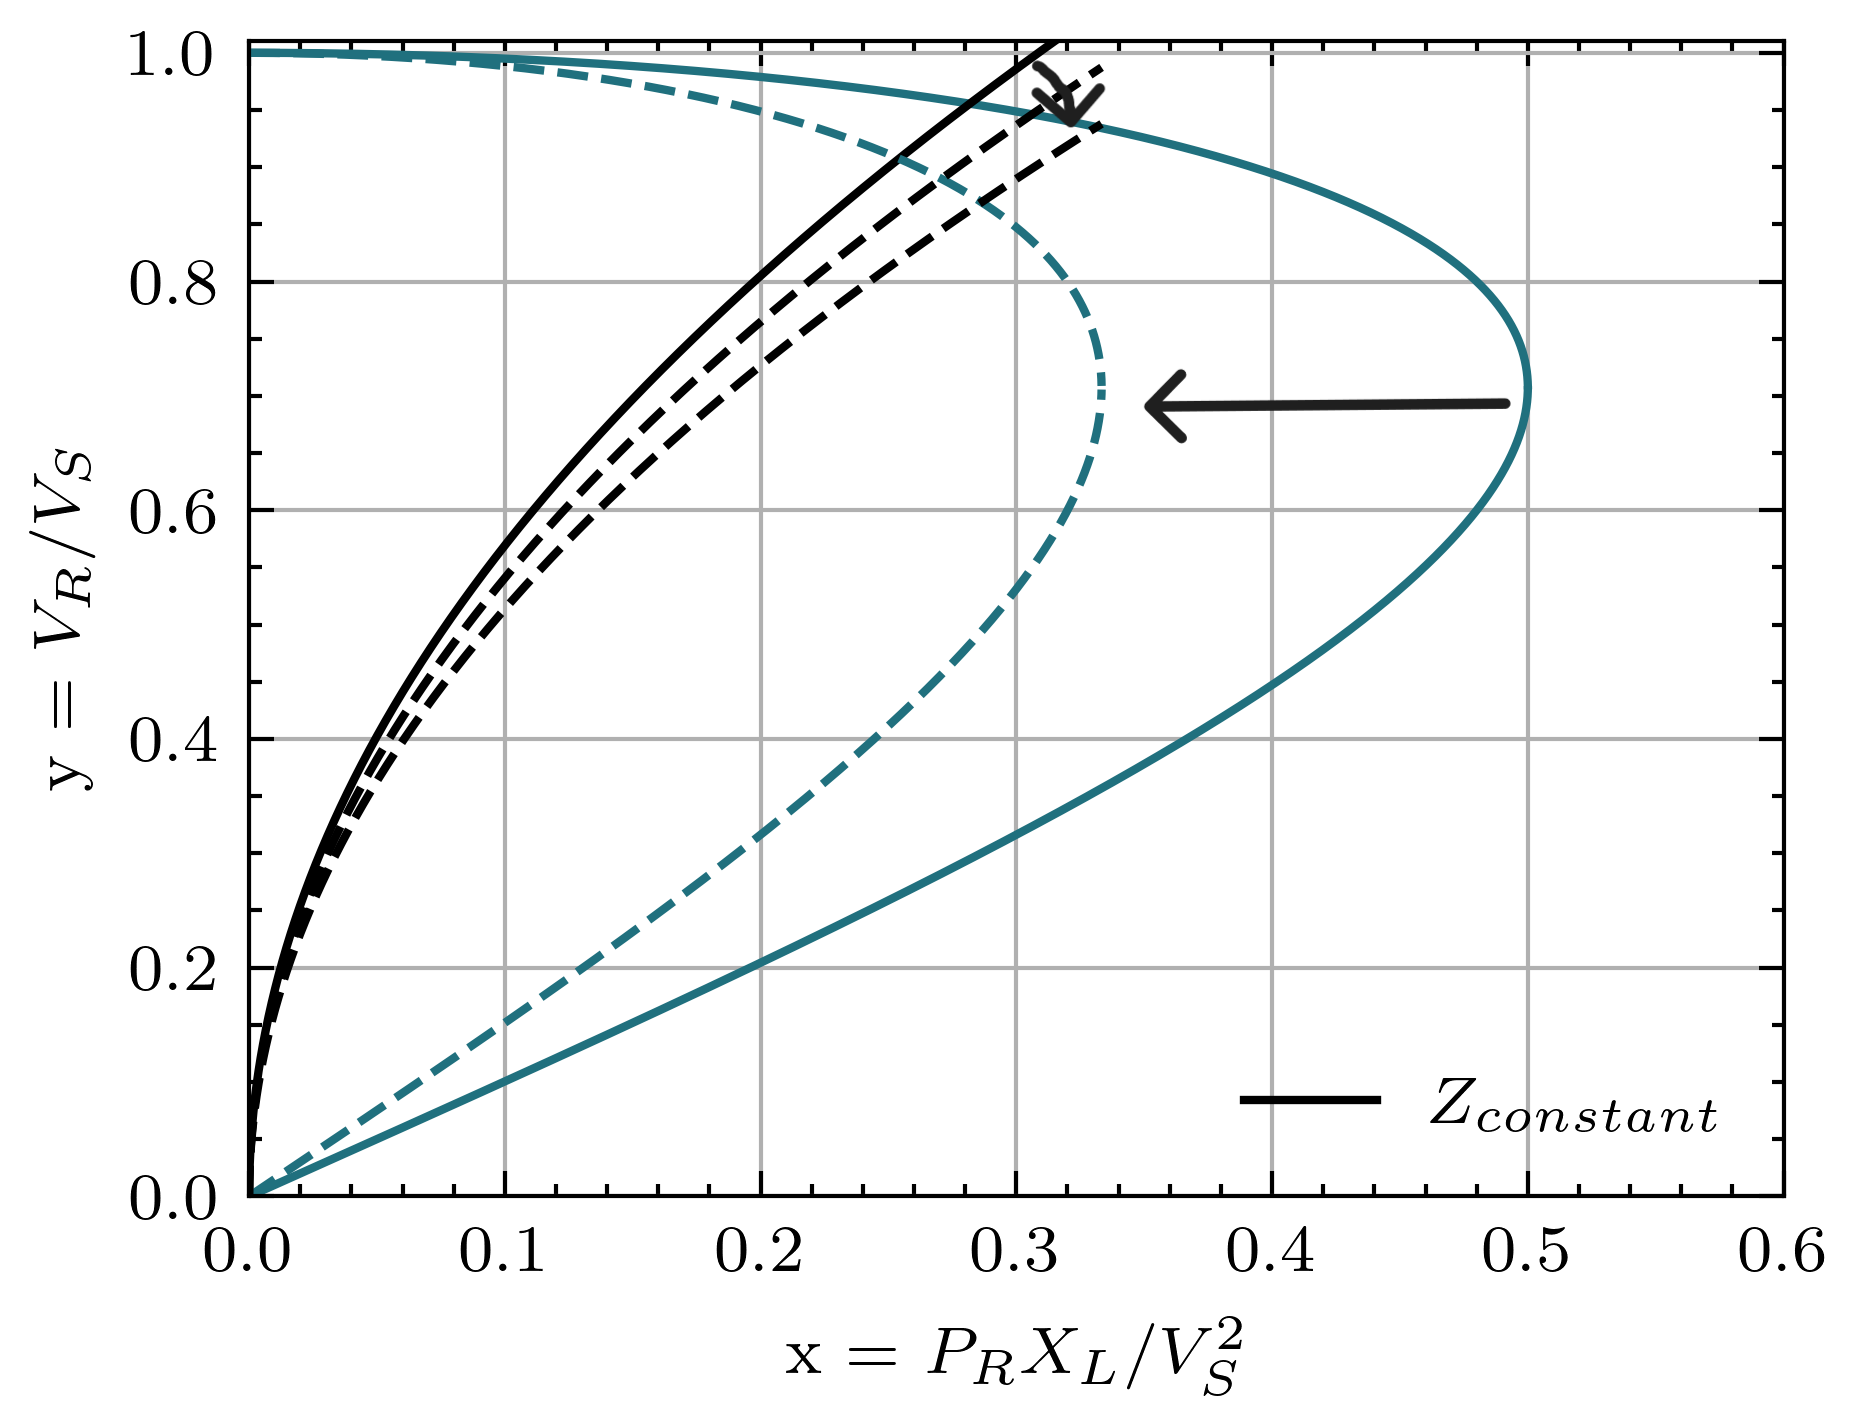
\includegraphics[width=0.45\textwidth]{images/PVcurvestable.png}
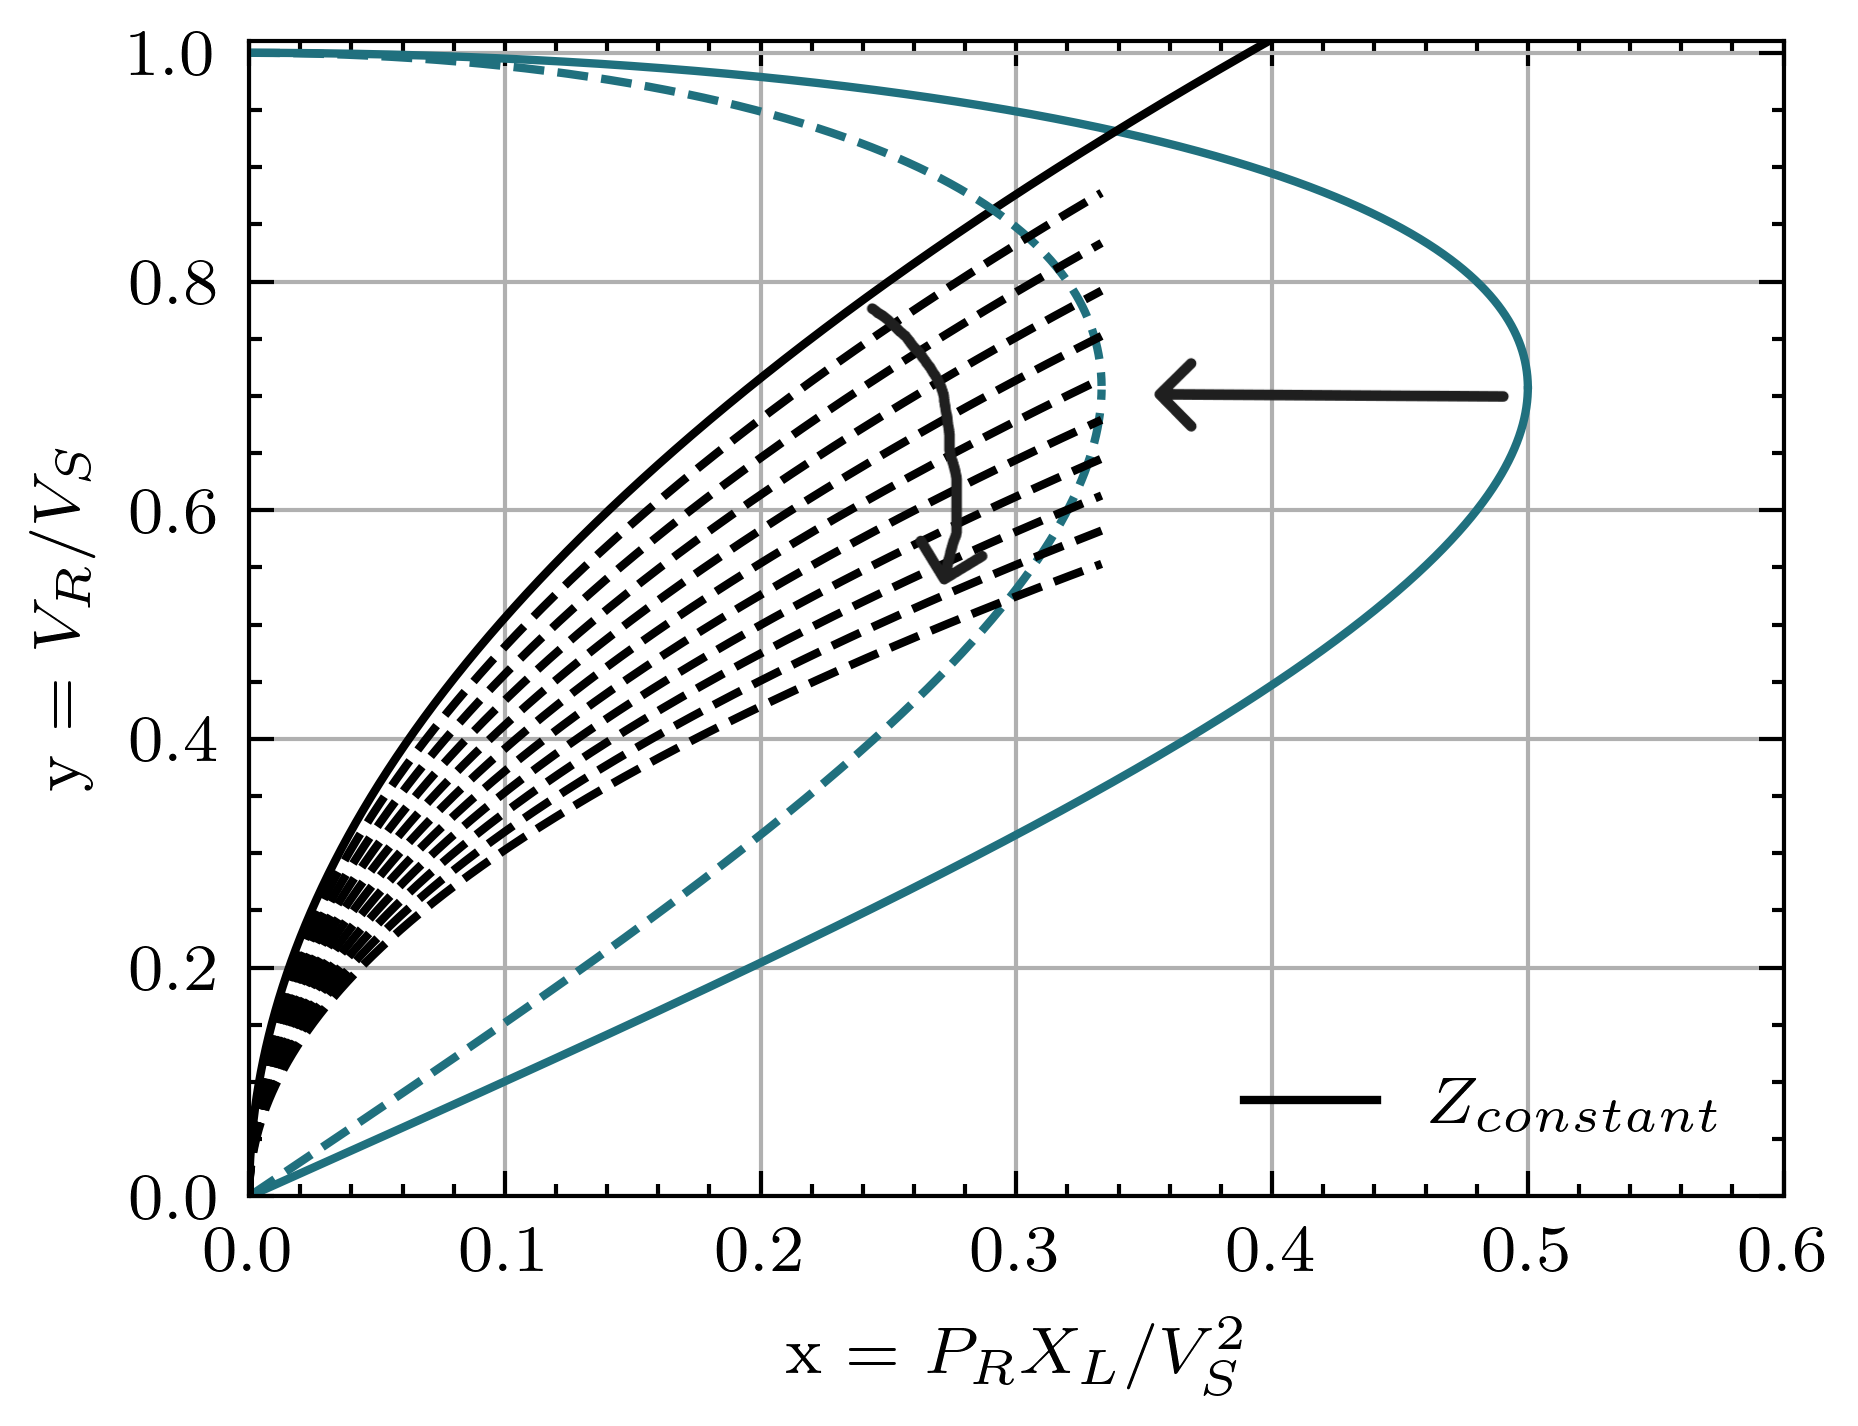
\includegraphics[width=0.45\textwidth]{images/PVcurveunstable.png}
\end{center}
\begin{itemize}
    \item 1) Left figure shows $P_G$ is recovered after two tap changes.
    \item 2) Right figure shows $P_G$ is never recovered, and the voltage collapses.
\end{itemize}
Scenario 2) is a typical case of \textbf{Long-term Voltage Stability}.
The disturbance can be the tripping of a line (as it is the case here), which leads to $X_L \nearrow$ or hitting the reactive power limits of a generator ($V_S$ is no longer maintained).
\end{frame}

\begin{frame} {Examples of voltage instabilities}
\emph{Short-term instabilities}
Consider an induction motor. The torque-speed curve is given below.
\begin{center}
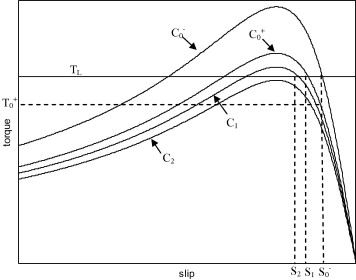
\includegraphics[width=0.5\textwidth]{images/Motorstalling.png}
\end{center}
$T_L$ is the mechanical torque. $C$ curves correspond to different electromechanical torques depending on the slip $s=\frac{\omega_s - \omega_r}{\omega_s}$.
The initial curve is $C_0^-$ and the machine operates on operating point $S_0$. If the voltage drops, the new curve becomes $C_0^+$.
The motor speed $\omega_r$ is reduced (thus $s$ increases), and we reach a new operating point $S_1$. This increase in $s$ leads to an increase in motor current and the further decrease in voltage and electrical torque. If the rate of decreasing voltage is slower than that of increasing slip, the voltage settles down.
\end{frame}

\begin{frame} {Examples of voltage instabilities}
If now the voltage drops faster, and the new curve becomes $C_2$, the motor speed is reduced until it completely stops (since there is no intersection between $C_2$ and $T_L$). The induction motor acts as a large inductance, drawing reactive power.
This is considered as a \textbf{Short-term Voltage Instability} as this phenomenon is much quicker than what we have with OLTCs (it takes several seconds to change tap positions). OLTCs are not able to restore the voltage.
\begin{center}
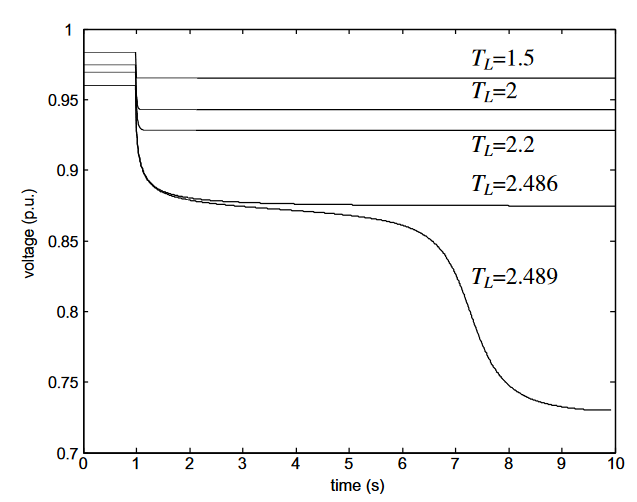
\includegraphics[width=0.6\textwidth]{images/InductionMotorVoltage.png}
\end{center}
\end{frame}




\section{Why do we need to control power systems?}

% Why and how to control voltage and frequency?
\begin{frame}{Why to control power systems?}
  \begin{itemize}
      \item Technical requirements: power system devices are designed so as to operate within well-defined "tolerance regions" 
      \begin{itemize}
        \item around nominal values of voltage $V_n$: $1 \pm 0.1$ pu in Europe
        \item around nominal value of frequency $f_n$: $50 \pm 0.2$  Hz in Europe (in steady state)
        \item within the $P$-$Q$ capabilities of devices
        \item under the current limits of lines and transformers
      \end{itemize} 
      \item Large/persistent deviations from nominal values could lead to 
      \begin{itemize}
        \item damages and safety problems (e.g. high voltage)
        \item cascading phenomena
        \item service interruptions
      \end{itemize}
      
  \end{itemize}
\end{frame}

\begin{frame}{Exogeneous threats}
  \begin{itemize}
      \item Sudden disturbances, such as line or generator tripping
      \item Fast variations of the \textit{net load} (cf. Duck curve)
      \begin{itemize}
        \item the net load refers to the load "seen" by the transmission system, i.e. the load minus the non-controllable dispersed generation
      \end{itemize}
      \item weather conditions, such as storms, which can impact the generation of renewable energy sources (RES) (e.g. wind turbines' cut-out speed)
  \end{itemize}
\end{frame}

% Principle of Automatic Voltage Control
\begin{frame}
    \frametitle{Principle of Automatic Voltage Control}
    \begin{itemize}
        \item \textit{The main tool:} primary voltage control via \textit{Automatic Voltage Regulators (AVRs)} of large synchronous generators and synchronous condensers
        \item Secondary voltage control and automatic switching of reactive compensation devices and transformer taps
        \item Tertiary voltage control and voltage profile optimization
    \end{itemize}
\end{frame}

% Automatic voltage regulator of a synchronous machine (reminder)
\begin{frame}
    \frametitle{Automatic voltage regulator of a synchronous machine (reminder)}
    \begin{columns}
        \begin{column}{0.35\textwidth}
            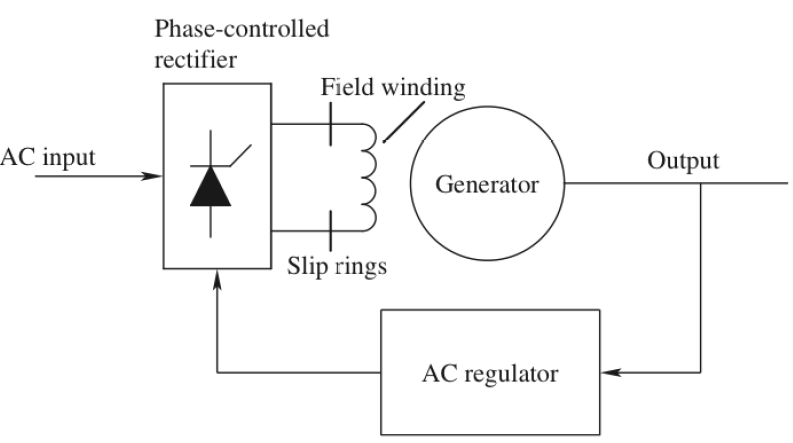
\includegraphics[width=\textwidth]{images/exciter.png}
        \end{column}
        \begin{column}{0.6\textwidth}
            \includegraphics[width=\textwidth]{images/avr.png}
        \end{column}
    \end{columns}
    \tiny{Figure on the right from: Voltage stability of electric power systems. T. Van Cutsem \& C. Vournas, KAP 1998}
    \begin{itemize}
        \item Notice that if several generators are connected in parallel (either at the MV or at the EHV bus), it is necessary to coordinate their AVRs so that they share the reactive power in an even way.
        \item The value of $Z_c$ may be adjusted in order to ensure such a coordination.
    \end{itemize}
\end{frame}

% Primary, secondary and tertiary voltage control
\begin{frame}
    \frametitle{Primary, secondary and tertiary voltage control}
    \begin{itemize}
        \item When a disturbance occurs, or subsequently to following the change in load (cf. 'duck curve'), the \textit{primary} voltage control loops maintain suitable voltage levels close to the large power plants equipped with AVRs.
        \begin{itemize}
            \item However, voltages at other buses may move out of tolerance intervals (in either direction), and reactive power reserves may not be shared in an even way among generators.
        \end{itemize}
        \item \textit{Secondary} voltage control loops can be used at the zonal level, to adjust the set-points of AVRs so as to control the voltage at 'pilot nodes' in the network while distributing the required reactive power evenly among generators.
        \begin{itemize}
            \item Secondary voltage control loops can also be used to switch shunt reactive compensation devices (capacitors/inductors) in order to increase reactive power generation margins in their zone (among a few large power plants).
        \end{itemize}
        \item \textit{Tertiary} voltage control uses OPF solvers to calculate set-points at pilot nodes and possibly adjust some transformer ratios, so as to minimize losses and maximize MVar reserves at the entire system level.
        \item Response times of different levels of voltage control
        \begin{itemize}
            \item \textit{Primary:} 1-3 seconds ; \textit{Secondary:} 30 seconds -3 minutes ; \textit{Tertiary:} 10-15 minutes
        \end{itemize}
    \end{itemize}
\end{frame}

\begin{frame}{Control resources}

    Which of these control resources are the main levers for freqency stability?
      \begin{itemize}
          \item Adjust synchronous generators' field current
          \item Adjust synchronous generators' mechanical power
          \item Change transformer taps
          \item Change shunt compensation
          \item Act on topology: switch lines and transformers in/out of service
          \item Fast start-up generator units
          \item In extremis load curtailment
          \item Control renewable generation (e.g. PV curtailment)
          \item Use batteries and other energy storage systems %TODO Ask ELIA to which reserve markets batteries are participating
      \end{itemize}
\end{frame}